\section{Literature Review}

The automation of mathematical tasks and reasoning has been pursued since at
least the time of mechanical calculators like the Pascaline~\cite{d'ocagne}. A
recurring theme in these efforts is the separation between those undertaken by
mathematicians like Pascal and Babbage~\cite{bowden}, and those of engineers
such as M\"uller~\cite[p. 65]{lindgren}. This pattern continues today, with the
tasks we are concerned with (automatically constructing and evaluating concepts,
conjectures, theorems, axioms, examples, etc.) being divided into two main
fields: Mathematical Theory Exploration (MTE)~\cite{buchberger:06} (also
sometimes prefaced with ``Computer-Aided'', ``Automated'' or
``Algorithm-Supported''), which is championed by mathematicians such as
Buchberger~\cite{buchberger}; and Automated Theory Formation
(ATF)~\cite{lenat:77,colton:book}, pursued by AI researchers including Lenat.
Other related terms include ``Automated Mathematical
Discovery''~\cite{epstein:91,colton2000notion,esarm2008},
``Concept Formation in Discovery Systems''~\cite{haase}, and
``Automated Theorem Discovery''~\cite{roy}.

Such a plethora of terminology can mask similarities and shared goals between
these fields. Even notable historical differences, such as the emphasis of MTE
on user-interaction and mathematical domains, in contrast to the full automation
and more general applications targeted by ATF, are disappearing in recent
implementations.

\subsection{Theory Formation}

An important historical implementation of ATF is Lenat's AM (Automated
Mathematician) system. Unlike prior work, such as
Meta-Dendral~\cite{buchanan:75} and those described in~\cite{winston}, AM aims
to be a general purpose mathematical discovery system, designed to both
construct new concepts and conjecture relationships between them. AM is a
rule-based system which represents knowledge using a frame-like scheme, enlarges
its knowledge base via a collection of heuristic rules, and controls the firing
of these rules via an agenda mechanism.

The performance of AM was evaluated based on its generality (performance in new
domains) and how finely-tuned various aspects of the program are (the agenda,
the interaction of the heuristics, etc). Most of this evaluation was
qualitative, and has subsequently been criticised~\cite[chap.~13]{colton:book}.
In their case study in methodology, Ritchie and Hanna found a large discrepancy
between the theoretical claims made of AM and the implemented
program~\cite{ritchie1984case}; for example, AM ``invented'' natural numbers
from sets, but did so using a heuristic specifically designed to make this
connection.

The successor of AM is Eurisko, a discovery system intended to be useful in more
general domains than just mathematical theory formation. Despite claiming some
early successes % FIXME Traveller TCS
work on Eurisko was put on hold due to a lack of machine-readable data about
real world systems for it to work with % FIXME Find something quotable
. This lead to the Cyc project, in an attempt to encode such knowledge in a
semantically rich and consistent form. Cyc is an ongoing project, with parts of
its database made available via OpenCyc.

\subsection{Theory Exploration}

The prototypical implementation of MTE is the Theorema system of Buchberger and
colleagues~\cite{buchberger,buchberger2016theorema}, which also places a strong
emphasis on user interface and output presentation. Theory exploration in the
Theorema system involves the user formalising their definitions in a consistent,
layered approach; such that reasoning algorithms can exploit this structure in
subsequent proofs, calculations, etc. The potential of this strategy was
evaluated by illustrating the automated synthesis of Buchberger's own Gr\"obner
bases algorithm~\cite{buchberger:04}.

A similar ``layering'' approach is found in the IsaScheme system of
Monta{\~n}o-Rivas \etal{}~\cite{Montano-Rivas.McCasland.Dixon.ea:2012}, which
has also been quantitatively compared against IsaCoSy and HipSpec using
precision/recall analysis~\cite{claessen2013automating}. The name comes from its
embedding in the Isabelle proof assistant and its use of ``schemes'':
higher-order formulae which can be used to generate new concepts and
conjectures. Variables within a scheme are instantiated automatically and this
drives the invention process. For example, the concept of ``repetition'' can be
encoded as a scheme, and instantiated with existing encodings of zero, successor
and addition to produce a definition of multiplication. The same scheme can be
instantiated with this new multiplication function to produce exponentiation.

IsaCoSy and QuickSpec (the conjecture generation component of HipSpec) are
described in more detail in $\S$\ref{sec:existing-tools}, since these are the
tools we chose to evaluate and compare for $\S$\ref{sec:application}. QuickSpec
has since evolved to version 2~\cite{smallbone2017quick}, which replaces the
distinct enumeration and testing steps with a single, iterative algorithm
similar to that of IsaCoSy. Generated conjectures are fed into a Knuth-Bendix
completion algorithm to form a corresponding set of rewrite rules. As
expressions are enumerated, they are simplified using these rules and discarded
if equal to a known expression. If not, QuickCheck tests whether the new
expression can be distinguished from the known expressions through random
testing: those which can are added to the set of known expressions. Those which
cannot be distinguished are conjectured to be equal, and the rewrite rules are
updated.

QuickSpec has also inspired another MTE tool for Haskell called
Speculate~\cite{braquehais2017speculate}, which operates in a similar way but
also makes use of the laws of total orders and Boolean algebra to conjecture
\emph{in}equalities and conditional relations between expressions.

Another notable MTE implementation, distinct from those based in Isabelle and
Haskell, is the MATHsAiD project (Mechanically Ascertaining Theorems from
Hypotheses, Axioms and Definitions)~\cite{roy}. Unlike the tools above, which
generate \emph{conjectures} that may later be sent to automated provers,
MATHsAiD directly generates \emph{theorems}, by making logically valid
inferences from a given set of axioms and definitions. Evaluation of the
interestingness of these theorems was performed qualitatively by the system's
developer, which highlights how these tools could benefit from the availability
of an objective, repeatable, quantitative method of evaluation and comparison
such as ours.

\section{Automated Software Improvement}

Software for analysing and improving code can be roughly divided into two
categories. Some contribute to the running of a program, such as (optimising)
compilers, linkers and interpreters. These must produce correct, predictable,
desirable results in a timely manner. For example, compiler optimisations should
not alter program semantics, should provide monotonic improvements in the
majority of cases (i.e. they should not be \emph{pessimisations}) and conditions
under which they apply should be predictable enough to prevent spurious
performance regressions when making seemingly innocuous
refactorings~\cite{robison2001impact}. Optimisations in ahead-of-time (AOT)
compilers must be fast enough to run during every build, and should have a large
enough impact on the generated code's performance that they
``pay for themselves''~\cite{Franz1994}; for just-in-time (JIT) compilers such
ideals become hard requirements, since any runtime transformation which doesn't
pay for itself is, by definition, a pessimisation.

The other category is that of ``standalone'' tools, which are run separately to
building or executing the target code, and whose results do not contribute
directly to the code's output. These include tools for testing, profiling,
verification, standards compliance, etc. The application of theory exploration
to software libraries fits into this latter category, whose constraints are not
as stringent as those applying to tools like compilers. The only real
restrictions on these tools are that their resource requirements are acceptable
to users, and that output is sufficiently high quality to be worth waiting for
and sifting through.

Some of the simplest code improvement tools are known as \emph{linters}, after
the \textsc{Lint} tool for the C programming language~\cite{Johnson78lint}.
Linters are standalone tools, characterised by parsing the given code and
looking for occurrences of certain syntax patterns; for example definitions
which are never used, ``no-op'' constructs (e.g. \texttt{if~(x~<~0)} when
\texttt{x} is of unsigned/non-negative type) and expressions which are valid but
usually used erroneously (e.g. \texttt{if (x = 1)} which performs assignment
rather than comparison).

A popular linter for Haskell is \textsc{HLint}~\cite{mitchell2014hlint}, which
focuses mostly on simplifying code; for example by spotting use-cases for common
library functions like \texttt{null x} instead of \texttt{length x == 0}.
Linting can be seen as the inverse of theory exploration: rather than inferring
novel, general relationships from patterns found in the code, linting begins
with known relationships and looks through the code for specific instances.
Whilst linting is a useful programming aid, and fast enough to apply regularly
(e.g. as a background process in a code editor), it is not an open-ended
process: once the predetermined patterns are exhausted, no more improvements
will be found.

At the other end of the code improvement spectrum we find
\emph{superoptimisers}~\cite{massalin1987superoptimizer}, which can take an
arbitrarily long time to find improvements, but whose deductive power is only
limited by the undecidability of the source language. Superoptimisers, such as
\textsc{Souper}~\cite{sasnauskas2017souper} and \textsc{Aha!} (``A Hacker's
Assistant'', developed to accompany \emph{Hacker's
  Delight}~\cite{warren2013hacker}) treat the given code as a specification, and
perform an open-ended search through the space of all programs to find the
optimal implementation according to some quality measure or cost model.

Supercompilers are often restricted to a branch- and effect-free subset of
machine code, where cost can be reasonably estimated by counting instructions or
cycles. Higher-level languages require more elaborate estimation methods, such
as cost semantics~\cite{danner2015denotational}: such models will still contain
many parameters, some of which may be determined by empirical measurement,
whilst others may depend on characteristics of the input data. Despite this
drawback, pareto-optimal optimisations can still be identified, and either
presented to the user or tested against a realistic data set (known as
\emph{profile-guided optimisation}~\cite{TODO}).

Superoptimisers also need some method to check whether a synthesised program
implements the required specification, such as a test suite and/or a theorem
prover. Proving correctness of machine code fragments is helped by the uniform,
finite nature of their domain (a fixed set of instructions, operating on a fixed
set of fixed-size registers). Higher level languages like Haskell are more
difficult to reason about and measure, since their behaviour and efficiency may
depend on unknown runtime parameters. In particular, optimising higher-order
functions is difficult in isolation, since many performance tradeoffs cannot be
decided without more knowledge of the functions involved. For example, a cache
of previous return values (known as a \emph{memo table}) can avoid re-computing
repeated calls to a function; but whether this actually saves time, or is worth
the memory penalty, depends on how long that function takes to calculate; and
how often it will be called with same arguments.

In addition to this uncertainty, each function's input domain may be infinite
(such as the natural numbers), and programs may use abstract interfaces and
datatypes with a variety of possible implementations (such as lists or key/value
mappings). All these factors makes effective testing more difficult, and proofs
potentially undecidable.

Even if these problems are mitigated, the biggest difficulty with
superoptimisation remains: the length of time it takes to search such a
large space. Whilst pruning methods can help~\cite{phothilimthana2016scaling},
the power of superoptimisation comes from its ``bottom up'' nature, which makes
no assumptions about the structure of the generated program. This generality is
expensive, with current superoptimisers typically scaling to code fragments only
a few dozen machine instructions long. Contemporary research has focused on the
use of stochastic search algorithms, such as Markov Chain Monte-Carlo (MCMC), to
synthesise promising improvements more quickly, whilst still finding optimal
implementations in the limit~\cite{schkufza2013stochastic}; guiding such
algorithms with \emph{learned} policies is also a promising area of
study~\cite{mudigonda2017learning}.

Rather than optimising individual units of code in isolation, we can instead
work ``top down'' and perform \emph{whole program optimisation}.\iffalse TODO: Cite MLTon, Stalin,
maybe others \fi In particular, for every function we may want to optimise, we
know \emph{all} call sites of that function within the program, and hence avoid
the need for a general solution. Statically-known values, including arguments to
(higher-order) functions, can be propagated through the code using techniques
like \emph{supercompilation}~\cite{Turchin:1986:CS:5956.5957}, and constant
expressions can be ahead of time; however this can dramatically increase code
size, as each function may be duplicated into multiple specialised instances.

Related techniques, like \emph{symbolic execution} (a form of \emph{abstract
  interpretation}), allow information to be statically deduced by tracing the
behaviour of code using an alternative execution model, where unknown runtime
data are represented as opaque metavariables. Property- and model-checkers are
similar, except they work dynamically by performing multiple runs, instantiating
metavariables with exhaustive or synthetic data (\quickcheck{} does this
randomly, \smallcheck{} enumerates values, etc.).

The most common code-improvement technique performed \emph{during execution} is
Just In Time (JIT) compilation~\iffalse TODO: Cite \fi, which allows an
interpreter to compile sections of code into a faster form (usually machine
code). Since this compilation takes time, it is usually reserved for sections
which are executed often enough to exceed some predefined threshold (e.g. 100).
By focusing on such ``hot paths'', the up-front costs of compiling everything
ahead of time are avoided; although compiled forms are kept only in memory,
getting recompiled as needed on each program run. Compiling at runtime also
allows specialisation with dynamically-known information; for example, inlining
specific implementations of a procedure rather than performing dynamic dispatch
(this is the problem higher-order functions discussed above). To avoid altering
semantics, such dynamic specialisations must be accompanied by a conservative
validity check (e.g. that the given arguments should use the procedure
implementation we have compiled-in), falling back to the interpreter upon
failure.

A more speculative use of optimisation during runtime has been proposed by
Hutter~\iffalse TODO: Cite \fi. As in a JIT-enabled interpreter, Hutter's
algorithm (also referred \hsearch{}) begins by directly executing the given
(unoptimised) program $p$ on the relevant input $x$ (this may be provided up
front, or piecemeal throughout execution, e.g. as a stream of user interaction
events). The variables $p_{fast}$ and $t_{fast}$ are initialised to $p$ and
$\infinity$ respectively, to indicate that $p$ is the fastest implementation we
have so far, and we don't yet have an upper bound on its running
time. Concurrently with the execution of $p$, two other processes are also
started:

\begin{itemize}
\item Process A searches for proofs (in a pre-specified formal system) that some
  program $p\prime$ is both semantically equivalent to $p$ and has a running
  time bounded by some other program $t$, i.e. for all inputs $i$, the
  time taken to compute $p\prime(i)$ is bounded by $t(i)$. A list is built up of
  the $(p\prime, t)$ pairs found so far.
\item Process B computes $t(x)$ for all of the bounds $t$ found so far by A.
  Computations are interleaved via a schedule similar to Levin's universal
  search algorithm~\iffalse TODO: Cite \fi, to prevent getting stuck on
  non-halting programs. Whenever a calculation of some $t(x)$ finishes, it is
  compared to $t_{fast}$: if smaller, $t_{fast}$ is set to $t(x)$, and $p_{fast}$ is
  set to $p\prime$ (the program paired with this $t$).
\end{itemize}

The execution of $p_{fast}(x)$ (initially $p(x)$) is restarted at
exponentially-spaced intervals: if the value of $p_{fast}$ gets updated,
execution will switch to the new, provably-faster program at the next restart.
Although wasteful, such restarting will only slow down execution by at most a
factor of 2; whilst switching to an updated $p_{fast}$ may bring arbitrarily large
speed-ups (depending on the problem). Since the proof search (process A) is
independent of the input $x$, it only contributes a constant factor to the
running time; although in the general case this factor will be exponential in
the length of the proof.

\hsearch{} is mostly of theoretical interest, being described as ``another $O()$
warning showing, how important [to running time] factors, and even subdominant
additive terms, are.''~\cite{TODO: Hutter, page 4}. Despite this caveat, the
general framework is still useful to compare with the code improvement
techniques described above. In particular, the use of open-ended search (process
A) is similar to that of superoptimisation; although the former enumerates
equivalence proofs and extracts programs from them, whilst the latter enumerates
programs and attempts to prove (or approximately determine)
equivalence. Likewise the speed estimation of process B is analogous to those
employed by superoptimisation. JIT compilation can also be achieved within this
framework, for example by including our desired optimisations in the axioms of
the formal system (making proof search trivial), biasing the search algorithm to
consider applications of these optimisations first, and including a simple cost
model for the language. Switching to faster programs can also be made
incremental, e.g. allowing (stateless) functions to be replaced individually
without having to restart execution, just like in a JIT-enabled interpreter.

The framework of the \goedelmachine{}~\cite{Schmidhuber:05icann} goes even
further than \hsearch{}: rather than limiting optimisations to just the given
program, it also searches for provable optimisations to \emph{itself}. In
principle, this allows the search algorithm, execution schedule, etc. to all be
optimised, replaced or even removed entirely, as long as a proof is found that
it would be beneficial to do so. The \goedelmachine{} concept is framed in the
language of reinforcement learning, with the goal of maximising``reward'' from
some ``utility function'', but it is easily to recast in terms of improving
efficiency: for example, choosing a utility function which provides a one-off
reward of $\frac{1}{t}$ if a result provably-equivalent to the original
program's is returned within $t$ steps; and 0 reward otherwise. The ability to
provide a utility function separate from the initial implementation is also
useful for specifying the desired task more declaratively: for example, if it is
acceptable to deviate from the behaviour of the initial implementation, as long
as some other criteria (given by the utility function) are satisfied. A relevant
example might be altering a search algorithm to find more results faster, even
if those aren't the same results that the original algorithm would have found.

The open-ended search through program and proof space performed by algorithms
like superoptimisation, \hsearch{} and the \goedelmachine{} are similar to that
of Theory Exploration (e.g. the discovery of equivalent expressions by
\isacosy{} and \quickspec{}). One major difference is in \emph{end result} of
these techniques: the latter tends to \emph{build up} structure and abstraction
latent in a set of definitions, whilst the former tend to \emph{tear down} such
layers to find direct, minimalistic implementations.

Another seeming contrast is that Theory Exploration has no specific ``target'',
unlike optimisers: it produces any properties found to match its
``interestingness'' criteria. However, the practical necessity of limiting
superoptimisers to only small snippets of code at a time has resulted in
applications like finding ``peephole optimisations''~\cite{Bansal.Aiken:2006},
whose scattershot nature is more akin to Theory Exploration than traditional
compiler optimisation. Likewise, the improvement in efficiency of an
optimisation (however that is measured or justified) contributes to its
interestingness, and hence suitability as an outputs for Theory Exploration
systems (especially in the use case of a programming assistant).

% TODO: Evolutionary patches

\subsection{Relevance Filtering}
\label{sec:relevance}

The combinatorial nature of formal systems causes many proof search methods,
such as resolution, to have exponential complexity
\cite{haken1985intractability}; hence even a modest size increase can turn a
trivial problem into an intractable one. Finding efficient alternatives for such
algorithms, especially those which are NP-complete (e.g. determining
satisfiability) or co-NP-complete (e.g. determining tautologies), seems
unlikely, as it would imply progress on the famously intractable open problems
of $\text{P} = \text{NP}$ and $\text{NP} = \text{co-NP}$. On the other hand, we
can turn this difficulty around: a modest \emph{decrease} in size may turn an
intractable problem into a solvable one. We can ensure that the solutions to
these reduced problems coincide with the original if we only remove
\emph{redundant} information. This leads to the idea of \emph{relevance
  filtering} (or, \emph{premise selection}, when viewed as the \emph{addition}
of relevant information to an initially-empty problem). This is the core idea
behind our restriction of theory exploration to intelligently-selected clusters
of symbols, rather than whole libraries at a time.

Relevance filtering has mostly been used in automated proof search, where it
simplifies problems by removing from consideration those clauses (axioms,
definitions, lemmas, etc.) which are deemed \emph{irrelevant}. The technique is
used in Isabelle's Sledgehammer tool, during its translation of Isabelle/HOL
theories to statements in first order logic: rather than translating the entire
theory, only a sub-set of relevant clauses are included. This reduces the size
of the problem and speeds up the proof search, but it creates the new problem of
determining when a clause is relevant: how do we know what will be required,
before we have the proof?

The initial approach taken by Sledgehammer, known as \textsc{MePo} (from
\emph{Meng-Paulson} \cite{meng2009lightweight}), gives each clause a score
based on the proportion $\frac{m}{n}$ of its symbols which are ``relevant''
(where $n$ is the number of symbols in the clause and $m$ is the number which
are relevant). Initially, the relevant symbols are those which occur in the goal
to be proved, but whenever a clause is found which scores more than a particular
threshold, all of its symbols are then also considered relevant. There are other
heuristics applied too, such as increasing the score of user-provided facts
(e.g. given by keywords like \texttt{using}), locally-scoped facts, first-order
facts and rarely-occuring facts. To choose $r$ relevant clauses for an ATP
invocation, we simply order the clauses by decreasing score and take the first
$r$ of them.

Recently, a variety of alternative algorithms have also been investigated, for
example the \textsc{MaSH} algorithm (Machine Learning for SledgeHammer)
\cite{kuhlwein2013mash} uses the ``visibility'' of one theorem from another to
determine the relevance of clauses. Visibility is essentially a dependency graph
of which theorems were used in the proofs of which other theorems (although the
theorems are actually represented as abstract sets of features). To select
relevant clauses for a goal, the set of clauses which are visible from the
goal's components is generated; this is further reduced by (an efficient
approximation of) a na\"{\i}ve Bayes algorithm.

Another example is \emph{multi-output ranking} (MOR), which uses a support
vector machine (SVM) approach for selecting relevant axioms from the Mizar
Mathematical Library for use by the Vampire ATP system
\cite{alama2014premise}. Many more approaches are described and evaluated in
\cite{kuhlwein2012overview}, some of which may be directly applicable in the
context of theory exploration.

\section{Interestingness}
\label{sec:interestingness}

A major challenge when generating conjectures is choosing how to focus attention
on only those deemed ``interesting'' (either by avoiding uninteresting search
paths, and/or by filtering down the eventual output), since this is an imprecise
term with many different interpretations. For example, all existing approaches
agree that simple tautologies are ``uninteresting'', but differ when it comes to
more complex statements.  Colton~\etal{} surveyed tools for theory formation
and exploration, and their associated notions of ``interestingness'', for
concepts and conjectures~\cite{colton2000notion}. Six qualities were identified,
which are applied to conjectured properties as follows:

{\bf Empirical plausibility} checks whether a property holds across some
specific examples. This is especially useful for avoiding falsehoods, without
resorting to a deductive proof search.

{\bf Novelty} depends on whether the property, or one isomorphic or more
general, has already been seen.

{\bf Surprisingness} of a property is whether or not it is ``obvious'', for
example if it is an instance of a tautology.

{\bf Applicability} depends on the number of models in which a
property holds. High applicability makes a property more interesting, but so
does zero applicability (i.e. non-existence).

{\bf Comprehensibility} depends on the syntactic complexity of the property's
statement. Simpler statements are considered more interesting (which favours
tools adopting a small-to-large search order).

{\bf Utility} is the relevance or usefulness of a property to the user's
particular task. For example, if we want to find properties which are useful for
optimisation, like Equation~\ref{eq:mapreduce}, then utility would include
whether the property justifies some rewrite rule, the difference in resource
usage of the expressions involved, and how common those expressions are in real
usage.

% FIXME: This is original work, so should maybe be in a different section
\begin{table}
  \centering
  \scalebox{0.9}{
    \begin{tabular}{ |l|l|c|c|c|c|c|c| }
      \hline
      \multirow{2}{*}{\textbf{Program}}                      &
      \multirow{2}{*}{\textbf{Conjecture Types}}             &
      \multicolumn{6}{c|}{\textbf{Interestingness Measures}} \\ \hhline{~~------}
      \tRow{             &                     & \iE & \iN & \iS & \iA & \iC & \iU}
      \tRow{AM           & \tIFF, \tIMP, \tNE  &   X &   X &   X &   X &   X &   X}
      \tRow{GT           & \tIFF, \tIMP, \tNE  &   X &   X &   X &   X &   X &   X}
      \tRow{Graffiti     & \tINE               &   X &   X &   X &     &   X &   X}
      \tRow{\Bagai{}     & \tNE                &     &   X &     &   X &   X &    }
      \tRow{HR           & \tIFF, \tIMP, \tNE  &   X &   X &   X &   X &   X &   X}
      \tRow{\quickspec{} & \tEQ                &   X &   X &     &   X &   X &    }
      \tRow{\speculate{} & \tCON\ \tEQ / \tINE &   X &   X &     &   X &   X &    }
      \tRow{\isacosy{}   & \tEQ                &   X &   X &     &   X &   X &   X}
      \tRow{\isascheme{} & \tEQ                &   X &   X &     &   X &   X &   X}
    \end{tabular}
  }
  \caption{Classification of MTE tools from~\cite{colton2000notion}, extended
    to include four more recent tools. The interestingness measures are
    \iE{}mpirical plausibility, \iN{}ovelty, \iS{}urprisingness,
    \iA{}pplicability, \iC{}omprehensibility (low complexity) and \iU{}tility.}
  \label{table:colton}
\end{table}

% JUSTIFICATIONS
%
% ICoSy uses counter-example checking; this ensures empirical plausibility
% ICoSy uses constraints to avoid special-cases; this ensures novelty
% ICoSy uses utility, since there are some hard-coded patterns which are
% looked for
%
% Speculat uses a form of unification to ensure novelty, making sure one
% equation is not a special-case of another
% Speculat uses LeanCheck to enumerate values, looking for counterexamples
% Speculat uses testing, to ensure Empirical Plausibility
%
% QSpec uses QCheck to ensure empirical plausibility
% QSpec uses a congruence closure algorithm to ensure novelty
%
% IScheme uses utility, since it determines the "quality" of a definition
% based on how many theorems it appears in?
% IScheme uses novelty, using an equational rewrite system (Knuth-Bendix
% completion) to remove redundancies
% IScheme uses utility, since it focuses on the terms and definitions of a
% user's theory. However, don't all of them?
% IScheme uses counterexample checking for empirical plausibility.

% ONLY APPLIES TO PRECONDITIONS
% APPLICABILITY: ensure a conjecture holds in many models (or exactly zero, in
% the case of Bagai et al). Does the testing-based approach of QuickSpec and
% Speculate ensure that there's a model? After all, these are concrete values
% rather than e.g. implications of some abstract specification.

% FIXME: Give brief description and reference for each system in the text.
% We could include the more lengthy descriptions of IsaCoSy and QuickSpec here?

We summarise the criteria in Table~\ref{table:colton} and state which were used
in key ATF/MTE tools. The entries for AM, GT, Graffiti, \Bagai{} and HR are
based on this survey (the latter is Colton's own tool). The remaining rows are
our extension of this analysis to the (higher-order) tools we have focused on
(based on our understanding of their function): \quickspec{}~\cite{QuickSpec},
\speculate{}~\cite{braquehais2017speculate},
\isacosy{}~\cite{Johansson.Dixon.Bundy:conjecture-generation}
and \isascheme{}~\cite{Montano-Rivas.McCasland.Dixon.ea:2012}.

These recent tools all use testing to check for counterexamples, which ensures
results are empirically plausible and applicable (conditions are satisfiable,
types are inhabited, etc.). They also use a small-to-large search order,
ensuring more easily-comprehensibile conjectures are explored first.

\isacosy{} ensures novelty using a constraint system to prevent special-cases
being generated, whilst the others use post-hoc filters based on unification and
term rewriting to achieve the same result. \isacosy{} is able to look for
commonly desirable patterns, such as commutativity and associativity, which
increases the utility of its output, whilst \isascheme{} is completely based
around such pattern-instantiation.

This diversity of approaches makes it difficult to compare the existing
evaluations of these tools directly. In particular, evaluation methods created
for one tool might not make sense for another, due to assumptions made about
the algorithms' operation. For example, the novelty filters used by \quickspec{}
and \speculate{} are applied to the whole output set, guaranteeing that no
special-cases will appear; yet we cannot assume this in the case of \isacosy{},
since its constraint solver allows special cases if they're found \emph{before}
the general case (it does not go back and discard previous results).

In addition, attempting to \emph{measure} these qualities directly is difficult,
and having too many measures complicates comparisons. System developers have
employed a more practical alternative in their evaluations, which is to perform
\emph{precision/recall} analysis against a \emph{ground-truth}. This requires
choosing a set of definitions and a set of properties (the ground truth) which
represent the ``ideal'' result of conjecture generation for those definitions.
To analyse the quality of a tool's conjectures, we run it on these chosen
definitions and compare its output to the ground truth:

\begin{itemize}
\item \emph{Precision} is the proportion of a tool's output which appears in
  the ground truth (the ratio of true positives to all positives). This
  penalises overly-liberal tools which output a large number of properties in
  the hope that some turn out to be ``good''.
\item \emph{Recall} is the proportion of the ground truth which appears in the
  tool's output (the ratio of true positives to actual positives). This
  penalises overly-conservative tools which generate very few properties as a
  way to avoid ``bad'' ones.
\end{itemize}

To score 100\% on precision and recall, all of the properties which appear in
the ground truth must have been conjectured, and nothing else. This gives us a
simple method to evaluate and compare tools without requiring a general solution
to the question of what is ``interesting''; although we must still decide what
to put in the ground truth set, and what to leave out, for each measured set of
definitions.

The precision/recall analysis shown in~\cite{claessen2013automating} is the only
quantitative comparison of recent MTE tools we have found in the literature.
Our Theory Exploration Benchmark, described in section~\ref{sec:benchmark}, is
essentially an extension of this approach, to a larger and more diverse set of
examples.

\subsection{Exploration in Theorem Proving}
\label{sec:examples}

Conjecture generation (automated or manual) is crucial when formally proving
statements, such verifying software against its specification. This provides a
concrete, empirical setting to determine what makes statements interesting (at
least from a utilitarian point of view).

\paragraph{Generalisation}

\providecommand{\coq}[1]{\lstinline[language=ML]|#1|}

When we \emph{generalise} a statement $S$, we obtain a new statement $S'$ of
which $S$ is a special case. Although it seems counterintuitive, a generalised
statement can sometimes be \emph{easier} to prove than the original. This arises
often in inductive proofs (e.g. when reasoning about tail-recursive
definitions~\cite{kapur2003automatic}\footnote{Tail-recursive functions are
  desirable due to their constant space usage, unlike recursion in non-tail
  positions which requires a growing number of stack frames or nested closures.
  The presence of accumulator arguments makes reasoning harder, so it is common
  to use the direct implementation for proofs, then transport them over to the
  tail-recursive definition via an equivalence relation.}), since the specific
obligations which arise in the proof may be incompatible with the available
inductive hypotheses. An informative example is given by Boyer and Moore of the
associativity of multiplication in \textsc{ACL2}~\cite{boyer1983proof}:

$$(x * y) * z = x * (y * z)$$

During the course of the proof, the following obligation arises:

\begin{equation}
  \tag{conc3}
  (y + (x * y)) * z = (y * z) + ((x * y) * z)
  \label{eq:conc3}
\end{equation}

ACL2 automatically generalises \eqref{eq:conc3} by replacing the repeated
sub-term $x * y$ with a fresh variable $w$:

\begin{equation}
  \tag{conc4}
  (y + w) * z = (y * z) + (w * z)
  \label{eq:conc4}
\end{equation}

This generalised form is clearly the distributivity law for multiplication and
addition, which can be proved separately to the original goal of
associativity. It would not be controversial to claim that this distributivity
law is interesting in its own right (relative to associativity, at least), in
addition to its usefulness in making this proof go through.

% TODO: Describe the ACL2 heuristics

Generality hence contributes to a conjecture's \emph{utility}, and also (by
definition) to its \emph{applicability}. It is still important to balance
against other concerns, since blindly generalising \emph{all} statements or
proof obligations we come across would result in conjectures so strong that they
are unprovable, or even false; which would make them much less interesting.

\paragraph{Analogy}

The interestingness of a statement can also be characterised by \emph{analogy}
to existing interesting statements. By finding lemmas analogous to those of a
different theory, we may be able to re-use proof tactics and other forms of
meta-programming across both. In this case an analogy would map from a solved
problem to a currently-unproven goal, and applying this map to the lemmas
appearing in the existing proof allows us to infer the approximate form of the
lemmas required for the new theorem.

The approach taken by \textsc{ACL2(ml)} is to find lemmas which may be relevant
to solving a goal $G$ by making analogies via unsupervised
clustering~\cite{Heras.Komendantskaya.Johansson.ea:2013}. These clusters are
used in two ways:

\begin{itemize}
\item First, we use the cluster $C_G$ containing $G$ to identify analogous
  theorems.

\item For each theorem $T \in C_G \setminus \{G\}$, we consider those symbols
  $S_T$ which occur in $T$ but not in $G$. Our analogous lemmas are those used
  to prove $T$, mutated such that symbols $s \in S_T$ are replaced by members of
  the cluster $C_s$ containing $s$.
\end{itemize}

The interestingness of such generated lemmas derives from both the existence of
the original lemma (which is presumably interesting enough to prove and
subsequently explore), that of the target theorem it may help to prove, and the
novelty provided by reframing existing concepts in a new domain. The running
examples for demonstrating \textsc{ACL2(ml)} are equivalence theorems for
tail-recursive definitions with their direct (non-tail-recursive) counterparts,
as well as the effect of repeating certain list operations:

\begin{itemize}
\item
  $\forall n, \texttt{natp}(n) \rightarrow \texttt{fact-tail}(n) =
  \texttt{fact}(n)$ where \texttt{natp} is the predicate that $n$ is a natural
  number, whilst \texttt{fact-tail} and \texttt{fact} are tail-recursive and
  non-tail-recursive implementations of factorial, respectively.

\item
  $\forall n, \texttt{natp}(n) \rightarrow \texttt{power-tail}(n) =
  \texttt{power}(n)$, where \texttt{power-tail} and \texttt{power} calculate
  powers of 2.

\item
  $\forall n, \texttt{natp}(n) \rightarrow \texttt{fib-tail}(n) =
  \texttt{fib}(n)$, where \texttt{fib-tail} and \texttt{fib} calculate fibonacci
  numbers.

\item
  $\forall x, \texttt{nat-listp}(x) \rightarrow \texttt{sort}(\texttt{sort}(x))
  = \texttt{sort}(x)$, for list-of-natural-numbers predicate \texttt{nat-listp}
  and list-sorting function \texttt{sort}.

\item
  $\forall x, \texttt{true-listp}(x) \rightarrow \texttt{rev}(\texttt{rev}(x)) =
  x$, where \texttt{true-listp} ensures that $x$ is a valid singly-linked list
  structure and \texttt{rev} is list reversal.

\item $\forall x, \texttt{true-listp}(x) \rightarrow \texttt{int}(x, x) = x$,
  where \texttt{int} is the intersection of lists (i.e. a list of elements
  common to each).
\end{itemize}

\paragraph{Auxiliary Lemmas} \label{sec:auxiliarylemmas}

One consideration when generating conjectures is the difference between
theorems, lemmas, corollaries, etc. From a logical point of view, these are all
equivalent, and hence most proof assistants do not distinguish between
them. However, their \emph{intention} may be different: in a sense, theorems are
the interesting results; whilst lemmas are useful results, required for proving
the theorems. Corollaries are consequences and special-cases of theorems, which
are interesting enough to state separately, but not as much as a theorem.

Some systems, like Coq, allow users to \emph{label} each statement as being a
\coq{Theorem}, a \coq{Lemma}, etc. despite their internal representations being
the same. This shows us immediately that lemmas outnumber theorems; in the Coq
standard library there are over five times as many lemmas as theorems
\footnote{Coq version \texttt{8.4pl6} contains (excluding comments) 1492
  occurences of \coq{Theorem} and 7594 of \coq{Lemma} in its \texttt{theories/}
  directory.}.

% TODO: Analyse them

% TODO: Theory exploration as lemma generation; give example from a HipSpec paper

We can find a need for auxiliary lemmas, once again, in the context of
tail-recursive functions. Consider proving the (pointwise) equality of the
following Coq functions, defined for the Peano naturals \coq{Z} and \coq{S}:

\begin{coqblock}
Inductive Nat : Set := Z : Nat
                     | S : Nat -> Nat.

Fixpoint plus      (n m : Nat) := match n with
                                      | Z    => m
                                      | S n' => S (plus n' m)
                                  end.

Fixpoint plus_tail (n m : Nat) := match n with
                                      | Z    => m
                                      | S n' => plus_tail n' (S m)
                                  end.
\end{coqblock}

These definitions are equivalent to the following Haskell:

\begin{haskell}
plus :: Nat -> Nat -> Nat
plus      Z      m = m
plus      (S n') m = S (plus n' m)

plus_tail :: Nat -> Nat -> Nat
plus_tail Z      m = m
plus_tail (S n') m = plus_tail n' (S m)
\end{haskell}

Both of these functions implement addition, but the \coq{plus_tail} variant is
tail-recursive. However, if we want to \emph{prove} that the definitions are
(pointwise) equal, we run into difficulties. In particular, when the inductive
step requires us to prove \coq{plus (S n) m = plus n (S m)} (which seems
reasonable), we cannot make this go through using another inductive argument.

\begin{coqblock}
(* Solve equalities by beta-normalising both sides *)
Ltac triv := try (simpl; reflexivity).

(* Prove equivalence of plus and plus_tail *)
Theorem equiv : forall n m, plus n m = plus_tail n m.
  induction n; triv. (* Base case is trivial *)

  (* Inductive case: plus (S n) m = plus_tail (S n) m *)
  intro m.

  (* Beta-reduce the right-hand-side (justification is trivial) *)
  replace (plus_tail (S n) m) with (plus_tail n (S m)); triv.

  (* Use induction hypothesis to replace plus_tail with plus *)
  rewrite <- (IHn (S m)).
\end{coqblock}

Specifically, the \emph{conclusion} of a second inductive hypothesis is exactly
the equation we need:

\begin{coqblock}
IHn' : (forall x, plus n' x = plus_tail n' x) -> plus (S n') m = plus n' (S m)
\end{coqblock}

Yet we cannot provide it with the argument it needs, as our original induction
hypothesis is \emph{too specific} (it has too many \coq{S} constructors):

\begin{coqblock}
IHn : forall x, plus (S n') x = plus_tail (S n') x
\end{coqblock}

We are forced to abandon the proof, despite such a reasonable-looking
intermediate goal.

In fact, if we attempt to prove that goal \emph{separately}, we can use a
straightforward argument by induction; even though it is actually
\emph{stronger} due to the absence of the \coq{IHn} assumption:

\begin{coqblock}
Lemma gen n m : plus (S n) m = plus n (S m).
  induction n; triv. (* Base case is trivial *)

  (* Move all S constructors outside *)
  simpl. rewrite <- IHn. simpl.

  (* Trivial *)
  reflexivity.
Defined.
\end{coqblock}

Using this separate result as a lemma, the orignal pointwise equality is proven
easily:

\begin{coqblock}
  rewrite (gen n m).
  reflexivity.
Defined.
\end{coqblock}

Hence demonstrating the utility, and therefore interestingness, of such
auxilliary lemmas.

% TODO Include Colton/Bundy et al

\subsection{Tests}

Since we are working in the domain of Haskell programs, an abundant source of
statements are available in the form of \emph{tests}. For manually-written
tests, the effort required to write them implies that they must be of some
interest to their author. Many forms of test are \emph{not} suitable for our
purposes, such as \emph{unit tests} which are always trivially provable by
$\beta$-reduction; or \emph{integration tests}, which depend on the behaviour of
the external environment. One reason to study Haskell is its widespread use of
\emph{property checking}, which does give us useful data in the form of
universally quantified statements. Many Haskell property checkers exist, based
on random testing (\quickcheck{}~\cite{claessen2011quickcheck} and
\smartcheck{}~\cite{pike2014smartcheck}), enumeration
(\smallcheck{}~\cite{runciman2008smallcheck}), observation
(\lazysmallcheck{}~\cite{reich2013advances}) and logic programming
(\sparsecheck{}~\cite{sparsecheck}).

Thankfully the major differences between these systems are in the way they
instantiate test arguments; their representations of properties are largely the
same (modulo renaming of functions and types): as Haskell functions with free
variables encoded as function arguments.

\subsection{Artificial Curiosity} \label{sec:intrinsic}

\begin{figure}
  \centering
  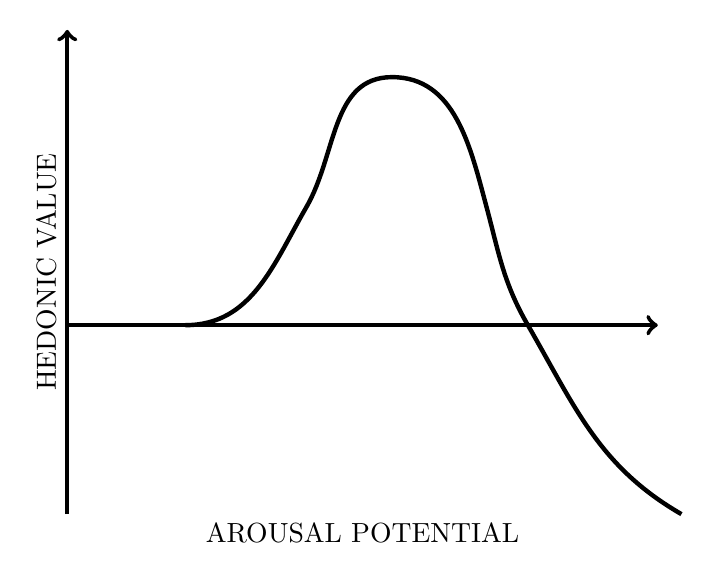
\begin{tikzpicture}[scale=0.75]
      % The image, for reference
      % \node[anchor=south west,inner sep=0] at (0,0) {\includegraphics[width=\textwidth]{wundt.png}};

      % Axes
      \draw[black,ultra thick,->] (1,0.8) -- (1,  9)   node[midway, above, sloped] {HEDONIC VALUE};     % y axis
      \draw[black,ultra thick,->] (1,4)   -- (11, 4);                                                   % x axis
      \path                       (1,0.8) -- (11, 0.8) node[midway, below]         {AROUSAL POTENTIAL}; % x axis label

      % Curve. The numbers come from tracing over wundt.png
      \draw[black,ultra thick] (3, 4)
           to[out=0,   in=240] (5.05, 6)
           to[out=60,  in=180] (6.5,  8.2)
           to[out=0,   in=105] (8.1,  6)
           to[out=-75, in=120] (8.8,  4)
           to[out=-60, in=150] (11.4, 0.8);

      % This version is closer, but a little jagged
      \iffalse
      \draw[black,ultra thick] (3, 4)
           to[out=0,   in=240] (5.05, 6)
           to[out=60,  in=225] (6,    8)
           to[out=45,  in=180] (6.5,  8.2)
           to[out=0,   in=135] (7.2,  8)
           to[out=-45, in=105] (8.1,  6)
           to[out=-75, in=120] (8.8,  4)
           to[out=-60, in=150] (11.4, 0.8);
      \fi
  \end{tikzpicture}

  \caption{The Wundt curve, reproduced from~\cite{berlyne1970novelty}. The axes
    ``hedonic value'' and ``arousal potential'' are described as covering
    \textquote{reward value\dots preference or pleasure}, and \textquote{all the
      stimulus properties that tend to raise arousal, including novelty and
      complexity}, respectively.}
  \label{fig:wundt}
\end{figure}

Another perspective on what is ``interesting'' comes from the artificial
intelligence tasks of optimisation and reinforcement learning. Common pitfalls
for such systems are highly non-convex problems (trapping optimisers in local
minima), and sparse information (such as flat gradients; or highly delayed
rewards, like a single win/lose reward at the end of a game). To mitigate these problems, various forms of internally-generated (or \emph{intrinsic}) rewards
can be incorporated into a system. Such schemes provide reward for interesting
discoveries, which encourages exploration in lieu of external direction, and are
known as \emph{Artificial Curiosity}~\cite{schmidhuber2006developmental} (AC).

The unifying principle of AC methods is to force systems away from data which
are not amenable to learning; either because they are so familiar that there is
nothing left to learn, or so unfamiliar that they are unintelligible. The
resulting behaviour is characterised by the \emph{Wundt curve} (shown in Figure \ref{fig:wundt}) \footnote{In practice, many measures
  avoid negative values for simplicity, in which cases we replace all negative
  points on the curve with zero.}, which has been used in psychology to explain
human aesthetics and preferences \cite{berlyne1970novelty}. This same behaviour
may be applicable to the theorems produced by a theory exploration system.

We can divide AC approaches into two groups: those which make \emph{explicit}
use of interestingness, learning from signals which follow a Wundt curve; whilst
\emph{implicit} approaches modify the \emph{output} of their learning
algorithm(s), to engineer the overall system behaviour to follow a Wundt curve
as an emergent property.

A framework encompassing many examples of the explicit approach is given
in~\cite{oudeyer2007intrinsic} in the context of reinforcement learning; for
comparison, many similar measures are surveyed in a data mining context
in~\cite{geng2006interestingness}. Many more reinforcement learning examples can
be found in~\cite{Kaplan2006, Lipson2007, Luciw2011, Macedo2000,
  Ramik.Sabourin.Madani:2013, Roa.Kruijff.Jacobsson:2009, Schmidhuber:1991,
  oudeyer2004intelligent}; whilst more general descriptions are given
in~\cite{Schaul.Sun.Wierstra.ea:2011, Scott1989, maher2008achieving}, which may
be more amenable to Theory Exploration setting.

Many of these reward signals are based on information theory, with a prominent
example being \emph{compression progress}: given a compressed representation of
our previous observations, the ``progress'' is the space saved if we include the
current observation. Observations which are incompressible or trivially
compressible don't save any space, whilst observations which provide new
insights into the structure of past experience can provide a space saving when
compressed together. This seems particularly relevant for identifying
interesting theorems: those new theorems (``observations'') which shorten the
proofs of previously discovered theorems may be more general, more powerful and
therefore more \emph{interesting}. In fact this is very similar to
\quickspec{}'s interestingness criterion.

Another example of explicit Artificial Curiosity is given
in~\cite{Hester.Stone:2012}, where world states which cause \emph{disagreement}
among a population of decision trees (a \emph{random
  forest}~\cite{randomforests}) are considered interesting. Since the models
make stochastic predictions, the disagreement follows a Wundt curve as the
complexity of state transitions increases: for parts of the state space which
have been fully learned, the models will agree on accurate predictions; for
parts which are unlearnable, the models cannot infer any structure, and will
converge to reporting the same average value. Whilst the latter predictions may
not be \emph{accurate}, they will be \emph{in agreement}, hence pushing down the
interestingness of states which are too complex.

Many examples of the implicit case are based on \emph{coevolution}: rewarding
one part of the system for exploiting another part, and vice versa. In~\cite{Schmidhuber1999} a pair of learning algorithms place virtual ``bets''
on the outcome of actions, and the winner is rewarded at the expense of the
loser. Due to the risk involved, each algorithm will only bet when it is
confident in its prediction, and bets will only be actioned when each algorithm
is confident in a \emph{different} outcome. The overall behaviour of this system
is therefore similar to the explicit measure of disagreement used in the random
forest example.

More recent work on \emph{Generative Adversarial Networks} (GANs) trains a
``discriminator'' program to distinguish real training examples (usually images)
from synthetic data made by a ``generator'' program. Both programs are
differentiable (usually some type of Artificial Neural Network), so the coupling
between the generator's output and the discriminator's input can be used not
only to feed synthetic data ``forwards'', but also to back-propagate the
discriminator's errors (which it is trying to minimise) into the generator
(which then tries to maximise, exploiting the discriminator by synthesising more
realistic data).

Another example of implicit AC is the ``darwinian brain'' of Fernando et
al.~\cite{fernando2013design1, fernando2013design2}. This coevolves a
population of problem generators and problem solvers, rewarding the solvers
based on their speed, and rewarding the generators based on the \emph{variance}
of the solvers' speed. This avoids trivial problems (which all solvers can
quickly overcome) and complex problems (which no solver can manage), and focuses
on those with the most possibility for learning. The role of problem generator
is similar to that of Theory Exploration tools, with solvers being Automated
Theorem Provers.

% TODO Include something about
% variance among experts (decision tree stuff as well as more established
% splitting functions stuff)

% TODO: Also mention the intrinsic reward idea about easily accessible regions
% (e.g. balancing a pole because it's easier to get from there to anywhere else)

% TODO Make sure we mention the recent reinforcement learning task that includes
% a constantly-changing "TV" in the 3D world, shown in some TwoMinutePapers
% videos

